\documentclass[a4paper, 5p, sort&compress]{elsarticle}%5p for double column
%
\usepackage{ucs}
\usepackage[utf8]{inputenc}
\usepackage{amsmath,amssymb,amsfonts,mathtools}
\usepackage[english]{babel}
\usepackage{fontenc}
\usepackage{graphicx}
%\usepackage[caption=false]{subfig}
\usepackage{ulem}
\usepackage[margin=0pt,font=footnotesize, labelsep=colon]{caption}
\usepackage{tabularx}
\usepackage{multirow}
\usepackage{units}
%\usepackage{subfig}
%\usepackage{siunitx}
\usepackage{booktabs}
\usepackage{bbm}
\usepackage{eurosym}
\usepackage{color}
\usepackage[table]{xcolor}
\usepackage{colortbl}
\usepackage{supertabular}
\usepackage{array,lipsum}
%\usepackage[author-year]{natbib}

\definecolor{rgrey}{gray}{0.75}
\newcommand{\mean}[1]{\langle #1 \rangle}
\newcommand{\E}[0]{\euro \;}
\newcommand{\bs}[1]{\boldsymbol{#1}}
\renewcommand{\rm}{\text }

% Added by emher
\usepackage[noabbrev]{cleveref}
\usepackage[export]{adjustbox}[2011/08/13]
\newcommand{\paren}[1]{\left(#1\right)}
\newcommand{\chromowidth}{1.00 \columnwidth}
\graphicspath{{Figures/}}
\usepackage{algorithm}
\usepackage[noend]{algpseudocode}
\usepackage{placeins}
\usepackage{subcaption}
\setlength{\parindent}{0pt}
\usepackage[toc,nonumberlist]{glossaries}
\usepackage{float}
\newfloat{algorithm}{H}{lop}
\floatname{algorithm}{Algorithm}
%\newfloat{algorithm*}{t}{lop}
%\floatname{algorithm*}{Algorithm}

%%%%%%%%%%%%%%%%%%%%%%%%%%%%%%%%%%%%%%%%%%%%%%%%%%%%%%%%%%%%%%%%
%%%%%%%%%%%%%%%%% Glossary setup %%%%%%%%%%%%%%%%%%%%%%%%%%%%%%%
%%%%%%%%%%%%%%%%%%%%%%%%%%%%%%%%%%%%%%%%%%%%%%%%%%%%%%%%%%%%%%%%

\newacronym{vres}{VRES}{Variable Renewable Energy Sources}
\newacronym{rea}{REA}{Renewable Energy Atlas}
\newacronym{ncep}{NCEP}{American National Centers for Environmental
  Prediction}
\newacronym{cfsr}{CFSR}{Climate Forecast System Reanalysis}

\newacronym{ac}{AC}{Alternating Current}
\newacronym{dc}{DC}{Direct Current}
\newacronym{lcoe}{LCOE}{Levelised Cost of Electricity}
%\newacronym{tfsc}{TFSC}{Thin-Film Solar Cell}
\newacronym{hvdc}{HVDC}{High Voltage Direct Current}
\newacronym{iset}{IWES}{Fraunhofer-Institut für Windenergie und Energiesystemtechnik}

\newacronym{ga}{GA}{Genetic Algorithm}
\newacronym{gas}{GAS}{Greedy Axial Search}
\newacronym{cs}{CS}{Cuckoo Search}
\newacronym{de}{DE}{Differential Evolution}

\newacronym{CapEx}{CapEx}{capital expenditures}
\newacronym{OpEx}{OpEx}{operational expenditures}

\begin{document}
\crefname{appendix}{}{}

%*************************************************
\begin{frontmatter}

\title{Optimal heterogeneity of a highly renewable pan-European electricity system}

\author[label1]{Emil H. Eriksen}
\ead{emher@au.dk}
%\author[label2]{Benjamin Sairanen}
\author[label2]{Tom Brown}
\ead{brown@fias.uni-frankfurt.de}
\author[label3]{Martin Greiner}
\ead{greiner@eng.au.dk}
\address[label1]{Department of Physics and Astronomy, Aarhus University, 8000 Aarhus C,  Denmark}
%\address[label2]{Department of Mathematics, Aarhus University, 8000 Aarhus C,  Denmark}
\address[label2]{Frankfurt Institute of Advanced Studies (FIAS), Johann Wolfgang Goethe Universit\"at, Ruth-Moufang-Straße 1, 60438 Frankfurt am Main, Germany}
\address[label3]{Department of Engineering, Aarhus University, 8200 Aarhus,  Denmark}



\begin{abstract}
  The resource quality and the temporal generation pattern of variable
  renewable energy sources vary significantly across Europe. Spatial
  distributions of renewable assets are explored which exploit this
  heterogeneity to lower the total system costs for a given level of
  renewable electricity in Europe. A local search algorithm as well as
  more intuitive heuristic algorithms are used to find optimal
  distributions of generation capacities that minimise backup,
  transmission and renewable capacity costs simultaneously. Using
  current cost projections, an optimal distribution favours onshore
  wind in countries bordering the North Sea, which results in average
  electricity costs that are up to 17\% lower than a homogeneous
  distribution of renewables proportional to each country's mean
  load. The sensitivities of the results to changing costs of solar
  generation and different mixes of onshore and offshore wind are also
  examined.

\end{abstract}

\begin{keyword}
renewable energy system \sep
levelised cost of electricity \sep
wind power generation \sep
solar power generation
\end{keyword}

\end{frontmatter}


%*************************************************************************
\section{Introduction}
\label{sec:one}
%*************************************************************************

The ambitious renewable energy targets set by European governments
\cite{eu2050} imply that the share of renewables in electricity
generation will increase significantly in the years to come.  The
electrification of other sectors, such as transportation, heating and
cooling, will also play a major role in the transition
\cite{Williams12,ecf2050}. At present, the leading renewable
technologies are wind, solar photovoltaics (PV) and hydroelectricity,
of which only wind and solar PV have the potential for large scale
expansion. For this reason, wind and solar PV
are focussed upon here.

Since wind and solar PV are both \gls{vres}, backup generation is needed if the electrical demand is to be met at all times. Backup
generation introduces additional system costs, which must be kept at a minimum.

The backup requirements depend on the mismatch between \gls{vres} generation and load. Using
the degrees of freedom associated with the choice of the capacity distributions of \gls{vres} for each country, it is
possible to smooth out the aggregated temporal generation pattern or even shape it towards the
load pattern. As a result, the mismatch (and thus the backup requirements) is lowered.  To
decrease the dimensionality of the problem, renewable assets are often assigned proportional to
the mean load of a country in accordance with a homogeneous wind-to-solar mixing factor. This
approach is demonstrated in \cite{Heide2010,Heide2011}, where optimal wind-to-solar mixes for
Europe are found that minimise balancing and storage costs.

Further reductions in backup requirements are possible by extending
the transmission network to enable more energy exchange between the
countries \cite{rolando2014,sarah}, but this must be balanced against the costs of transmission infrastructure. Other relevant research on the
advantages and costs of grid extensions can be found in
\cite{Papae,Schaber,Schaber2,Egerer,Brown}.

% PUT IN 2050 report stuff here?

In this paper the assumptions of a homogeneous spatial distribution of
\gls{vres} and a homogeneous wind-to-solar mixing factor are lifted and the
cost-optimal siting of \gls{vres} capacities around Europe is explored.

The distribution of \gls{vres} plants is determined by at least two considerations.
The first consideration is the geographical
variation of the \gls{vres}
quality. %On average, a solar photovoltaic (PV) installation in
% Spain will be more productive than an equivalent installation in
% Ireland. On the other hand, a wind farm located in Ireland will be
% productive than an equivalent installation in Spain.
The resource quality is quantified through the capacity factor (CF) defined as

\begin{equation}
  \label{eq:1}
  \mbox{CF} = \frac{\mbox{Average generation}}{\mbox{Rated capacity}} .
\end{equation}

The capacity factor is a number between 0 and 1, where 0 means no
generation and 1 means maximum generation at all times. Capacity
factors for the European countries for onshore wind, offshore wind and
solar PV are listed in \cref{tab:capacity-factors}.
%Wind turbines produce when it is windy, solar
%PV when it is sunny. Backup is thus needed at windless
%nights.

The second consideration is the geographical variation of the temporal generation pattern for a
given \gls{vres} type. This effect is particularly important for wind since Europe is large
compared to the correlation length of wind % of $\approx$ 1000 km
\cite{Widen2011}, and wind therefore benefits from smoothing effects across the
continent. Similar to the optimal wind/solar mixes found in \cite{Heide2010,Heide2011}, optimal
layouts of each \gls{vres} can be derived that, for example, reduce balancing or transmission
needs.

With these points in mind, the optimal heterogeneous spatial layouts
of wind and solar PV across Europe is investigated and compared to the
homogeneous layouts. The main point of comparison is the average cost
of electricity, which is composed of the transmission, backup and
\gls{vres} costs.  Different approaches to cope with the resulting
large number of degrees of freedom are considered. In contrast to
others who have used linear programming to
optimise generation and transmission capacities simultaneously
\cite{Czisch,Scholz,Hagspiel}, in this paper more intuitive heuristic
methods are developed to construct layouts based on knowledge of
resource quality, which are then compared to layouts obtained
through optimisation. For the optimisation a
local search algorithm was found to be most effective given the size
and non-linear formulation of the optimisation problem considered here.



%\textcolor{orange}{Two previous papers \cite{Rombauts11,Roques09} have applied
%Optimal Layout Theory to explore heterogeneous distributions of
%wind resources. They have found that there is a significant decrease
%in the overall risk, or standard deviation, when increasing the
%aggregation region, suggesting that there are benefits in establishing
%a transmission network, as also shown by \cite{Rodriguez2013}. In
%\cite{Elliston}, an out-of-the-box genetic algorithm has been applied
%to find the least-cost scenario for a highly renewable electricity
%system in the Australian National Electricity Market (NEM). They found
%that the least cost scenario was that with a penetration of around
%60\% renewables, consisting of around 70\% wind energy.}

% MAYBE MOVE THIS TO SOMEWHERE ELSE?

% The $\beta$ and CF layouts are derived directly from the capacity
% factor. They do not take the temporal production pattern into
% account. By choosing \gls{vres} with different temporal patterns, it is
% possible to reduce the backup needs. For homogeneous layouts, the
% dimensionality of the problem is two (one if $\gamma$ is fixed), and the
% optimum is trivially found. In the heterogeneous case, the
% dimensionality of the problem is 2N. For the 30-node network at hand
% 2N = 60 and the optimization no longer trivial. The quest for optimal
% layouts inside the 60 dimensional search space is the topic of
% \cref{sec:cuckoo-search}.

This paper is organised as follows: \Cref{sec:two} discusses the
general modelling of the electricity system, the key metrics and the
construction of heterogeneous layouts. In \cref{sec:results} the
performance of the different layouts and the resulting renewable
penetrations for individual European countries are
discussed. \Cref{sec:sensitivity-analysis} contains an analysis of the
sensitivity of the results to reductions in solar costs and to
expansions in offshore wind capacities. We conclude the paper with a
discussion on the results and an outlook on future research.

%*************************************************************************
\section{Methods}
\label{sec:two}
%*************************************************************************


\subsection{Renewable resource assessment}

Hourly time series for the generation of onshore wind, offshore wind and solar PV for each
European country were calculated using the \gls{rea}. The \gls{rea} time series are based on a
weather data set called the \gls{cfsr} from \gls{ncep} \cite{Saha}. The data set covers the period
from January 1979 to December 2010 and is available globally at an hourly temporal resolution
and a spatial resolution of $0.31^\circ \times 0.31^\circ$.

When creating time series on a country-wise basis, the capacity
factors depend strongly on the distribution of \gls{vres} in each
country. While the highest capacity factor would be obtained by
allocating all \gls{vres} to the best location, this is usually not
possible due to space limitations and political concerns. However,
since the capacity factor has a huge impact on the energy production
costs, a homogeneous distribution is not realistic either. As an
intermediate solution, the \gls{vres} layout was chosen as a
homogeneous distribution across the 50\% best grid points in each
country.

For wind conversion, a multi turbine
corrected power curve for the Vestas V90 3.0~MW turbine at 80 meter
hub height was assumed \cite{REA}. For solar conversion, the Solar First Series 4
PV panel oriented south and tilted from horizontal to a degree equal
to the latitude of installation was applied. % TODO: Add reference

The resulting capacity factors for each country and each technology are listed in
\cref{tab:capacity-factors}.


\begin{table*}[t!]
  \caption{Capacity factors $\text{CF}_n^w$, $\text{CF}_n^{\tilde{w}}$ and  $\text{CF}_n^s$ for onshore wind, offshore wind and solar PV for the European countries.}
  \label{tab:capacity-factors}
  \begin{adjustbox}{center}
    \begin{tabular}{lccclccclccc}  \toprule
      & $\text{\textbf{CF}}_n^w$ & $\text{\textbf{CF}}_n^{\tilde{w}}$ & $\text{\textbf{CF}}_n^s$ &  & $\text{\textbf{CF}}_n^w$ &
      $\text{\textbf{CF}}_n^{\tilde{w}}$ & $\text{\textbf{CF}}_n^s$ &  & $\text{\textbf{CF}}_n^w$ & $\text{\textbf{CF}}_n^{\tilde{w}}$ &
      $\text{\textbf{CF}}_n^s$\\ \midrule
      AT & 0.13 & - & 0.16 & DE & 0.20 & 0.44 & 0.14 & NO & 0.25 & 0.36 & 0.13\\
      BE & 0.22 & 0.40 & 0.14 & GB & 0.32 & 0.44 & 0.13 & PL & 0.17 & 0.34 & 0.14\\
      BA & 0.13 & - & 0.18 & GR & 0.14 & 0.34 & 0.19 & PT & 0.18 & 0.20 & 0.20\\
      BG & 0.12 & 0.19 & 0.18 & HU & 0.12 & - & 0.17 & RO & 0.11 & 0.24 & 0.18\\
      HR & 0.17 & 0.23 & 0.18 & IE & 0.35 & 0.38 & 0.11 & RS & 0.09 & - & 0.18\\
      CZ & 0.15 & - & 0.16 & IT & 0.13 & 0.17 & 0.19 & SK & 0.12 & - & 0.16\\
      DK & 0.37 & 0.45 & 0.13 & LV & 0.23 & 0.34 & 0.13 & SI & 0.07 & - & 0.16\\
      EE & 0.26 & 0.32 & 0.13 & LT & 0.20 & 0.32 & 0.13 & ES & 0.15 & 0.21 & 0.20\\
      FI & 0.18 & 0.33 & 0.11 & LU & 0.19 & - & 0.14 & SE & 0.21 & 0.32 & 0.13\\
      FR & 0.20 & 0.34 & 0.17 & NL & 0.27 & 0.43 & 0.13 & CH & 0.13 & - & 0.18\\ \bottomrule
    \end{tabular}
  \end{adjustbox}
\end{table*}


\subsection{The electricity network}
\label{sec:network}

The European electricity network is modelled using a simplified
30-node model, where each node represents a country (see \cref{fig:links} for the layout of the network). The nodal load is
determined from historical data, while wind and solar generation data
are calculated using a combination of weather data and physical models
\cite{REA}. Initially, wind is assumed to be onshore only. For each
node $n$ the generation from \gls{vres},

% -------------------
\begin{equation}
  G^{R}_{n}(t) = G_{n}^{W}(t) + G_{n}^{S}(t),
\end{equation}
% -------------------

can be expressed through two parameters. The penetration $\gamma$
determines the amount of energy generated relative to the mean load of
the node,

% -------------------
\begin{equation}
  \mean{G^{R}_{n}} = \gamma_{n} \mean{L_{n}} ,
\end{equation}
% -------------------

while the mixing parameter $\alpha$ fixes wind-to-solar ratio,
%-------------------
\begin{align}
  \mean{G^{W}_{n}} &=  \alpha_{n} \mean{G_{n}^{R}}  , \\
  \mean{G^{S}_{n}} &=  \paren{1- \alpha_{n}} \mean{G_{n}^{R}}  .
\end{align}
%-------------------

The nodal difference between \gls{vres} generation and load

%-------------------
\begin{equation}
  \Delta_{n}(t) = G^{R}_{n}(t) - L_{n}(t)
\end{equation}
%-------------------

is called the mismatch. To avoid power outages, the demand must be
met at all times. Since storage is not considered, any power
deficits must be covered by backup generation. Dispatchable
resources are not modelled explicitly, but are considered a part of
the backup generation. If $\Delta_{n}(t) \geq 0$, excess energy must be
curtailed $C_{n}(t)$, while if $\Delta_{n}(t) < 0$ backup generation
$G^{B}_{n}(t)$ is needed.
% -------------------
%\begin{align}
%  C_{n}(t) &= + \max \paren{\Delta_{n}(t),0} \\
%  G^{B}_{n}(t) &= - \min \phantom{} \paren{\Delta_{n}(t),0}
%\end{align}
% -------------------
Together the two terms form the nodal balancing
$B_{n}(t) = C_{n}(t) - G^{B}_{n}(t)$.
%
It is possible to lower the balancing needs with transmission. Nodes
with excess generation export energy $E_{n}(t)$, allowing nodes with
an energy deficit to import energy $I_{n}(t)$ to (partly) cover their
energy deficit. The nodal injection, $E_{n}(t) - I_{n}(t)$, is denoted
$P_{n}(t)$. This leads to the nodal balancing equation,

% -------------------
\begin{equation}
  \label{eq:nodal-balancing}
  G^{R}_{n}(t) - L_{n}(t) = B_{n}(t) + P_{n}(t), % + S_{n}(t) ,
\end{equation}
% -------------------

The vector of nodal injections $\mathbf{P}$ is called the injection
pattern. The actual imports and exports, and thus the injection
pattern, depend on the dispatch of the nodal balancing. It is
convenient to express the dispatch rules in terms of a two step
optimisation problem. The top priority is to minimise the backup
generation for each time step,

% -------------------
\begin{equation}
  \label{eq:step1}
  \begin{aligned}
    \text{Step 1: \hspace{15pt}}& \underset{\mathbf{P}, \mathbf{F}}{\text{min}}
    & & \sum_{n} \frac{\paren{B_{n}(t)}^{2}}{\mean{L_{n}}} \\
    & \text{s.t.}
    & & \sum_{n} P_{n} (t) = 0 \\ %F_{l}^{-} \leq F_{l} \leq F_{l}^{+}
    & \text{s.t.}
    & & F_{l}^{-} \leq F_{l} (t) \leq F_{l}^{+}
  \end{aligned}
\end{equation}
% -------------------

where $F_{l}$ is the flow on link $l$ and $F_{l}^{\pm}$ denote flow
constraints. By minimising $B_{n}^{2}$ (divided by $\mean{L_{n}}$)
rather than $G_{n}^{B}$, the particular solution where all nodes are
curtailing/generating backup synchronously (relative to
$\mean{L_{n}}$) is obtained
\cite{Rolando2015}. %While \cref{eq:step1} fixes \textbf{P}, the problem remains
%degenerate in \textbf{F}. As an example, if \textbf{F'} is a solution,
%any solution \textbf{F''} obtained by adding a circular flow to
%\textbf{F'} will also be a solution. The degeneracy is removed by a
%second optimization step.
To ensure that the resulting flow obeys the physical flow equations, the
objective in the second step is chosen to minimise the sum of squared flows
\cite{Magnus}.

% -------------------
\begin{equation}
  \begin{aligned}
    \label{eq:step2}
    \text{Step 2: \hspace{15pt}} & \underset{\mathbf{F}}{\text{min}}
    & & \sum_{l} F_{l}(t)^{2} \\
    & \text{s.t.}
    & & \mathbf{P}(t) = \mathbf{P}^{*}(t) \\ %F_{l}^{-} \leq F_{l} \leq F_{l}^{+}
    & \text{s.t.}
    & & F_{l}^{-} \leq F_{l}(t) \leq F_{l}^{+} \\
    %& \text{s.t.}
    %& & G_{n}^{B} = G_{n}^{B*} ,
  \end{aligned}
\end{equation}
% -------------------

where $\mathbf{P}^{*}$ is the injection pattern found in step 1.

%\footnote{This is only strictly true for unconstained
  %flow. However, even when flow constraints are present, the minimal
  %flow solution represents a fairly good approximation\cite{Magnus}.}.

\subsection{Key metrics}
\label{sec:key}


Following \cite{Sensitivity}, the energy system cost is calculated
based on a few key parameters. Besides the cost of the \gls{vres}
capacities, $\mathcal{K^{W}}$ and $\mathcal{K^S}$, costs for the
backup system and the transmission network are included. The backup
system cost is split into two components, the cost of backup capacity
$\mathcal{K}^{B}$ and the cost of backup energy $E^{B}$. The backup
capacity cost covers expenses related to construction and to keeping
the power plants online while the backup energy cost accounts for
actual fuel costs. Expressed in units of the average annual load, the
backup energy is given by

% -------------------
\begin{equation}
  \label{eq:backup-energy}
  E^{B} =\frac{\sum_{n} \sum_{t} G^{B}_{n}(t)}{\sum_{m} \sum_{t}
    L_{m}(t)} = \sum_{n} \frac{\langle G^{B}_{n} \rangle}{\langle L_{n}
    \rangle} .
\end{equation}
% -------------------

In principle, the backup capacity is fixed by a single extreme
event. However with this definition, the results will be highly
coupled to the particular data set used. To decrease the coupling, the
99\% quantile is used rather than the maximum value,

\begin{equation}
  \label{eq:2}
  q_{n} = \int _{0} ^{K_{n}^{B}} p_{n}(G^{B}_{n})dG^{B}_{n},
\end{equation}

where $p_{n}(G^{B}_{n})$ is the time sampled distribution of backup
generation and $q_{n} = 0.99$. With this choice, the backup system
will be able to cover the demand 99\% of the time. The remaining 1\%
is assumed to be covered by unmodelled balancing initiatives,
e.g. demand side management. Given the nodal values
$\mathcal{K}^{B}_{n}$, the overall backup capacity

\begin{equation}
  \label{eq:4}
  \mathcal{K}^{B} = \sum_{n} \mathcal{K}^{B}_{n}
\end{equation}

is calculated by summation. In analogy, the transmission capacity $\mathcal{K}^{T}_{l}$ is defined
so that the flow is met 99\% of the time. Transmission can be
positive and negative, but since links are assumed bidirectional, only
the magnitude (not the sign) of the flow is to be considered. Hence

\begin{equation}
  \label{eq:link-cap}
  q_{l} = \int _{0} ^{K_{l}^{T}} p_{l}(|F_{l}|)dF_{l},
\end{equation}

where $p_{l}(|F_{l}|)$ is the time sampled distribution of absolute
flows and $q_{l} = 0.99$. Since the link length varies,
$\mathcal{K}^{T}$ is not calculated directly by summation, but instead
as a weighted sum,

\begin{equation}
  \label{eq:4}
  \mathcal{K}^{T} = \sum_{l} \mathcal{K}^{T}_{l} d_{l},
\end{equation}

where $d_{l}$ denotes the length of link $l$.

In this paper $E^{B}$ will be expressed in units of average annual
load, $\mathcal{K}^{B}$ in units of average hourly load and
$\mathcal{K}^{T}$ in units of average hourly load $\times$ megametre.

\subsection{Cost modelling}
\label{sec:cost-modelling}

Cost assumptions for the elements of an electricity system vary
greatly across the literature \cite{Sensitivity}. In this study, the
cost assumptions published by \cite{Rolando} have been adapted with a
single modification. The cost of solar has been reduced by 50\% in
accordance with near future solar PV panel price projections
\cite{irena}. The resulting estimates are listed in
\cref{tab:cost-assumptions}. In general, the cost assumptions are in
the low end for \gls{vres} which reflects the expectation that the cost of
\gls{vres} will go down in the future as the penetration increases
\cite{Fraunhofer}.  Backup generation is priced based on the cost of Combined Cycle Gas Turbines (CCGTs).

\begin{table}[h!]
  \centering
  % Note: Text is missing in the caption (it was "outside" of the scan).
  \caption{Cost assumptions for different assets separated into
    \gls{CapEx} and fixed/variable \gls{OpEx}.}
  \label{tab:cost-assumptions}
  \begin{tabular}{lrrr}  \toprule
    \textbf{Asset} & \textbf{\gls{CapEx} }& \textbf{\gls{OpEx}$_{\text{fixed}}$} & \textbf{\gls{OpEx}$_{\text{variable}}$}\\
    & [\euro/W] & [\euro/kW/y] & [\euro/MWh]\\ \midrule
    CCGT & 0.90 & 4.5 & 56.0\\
    Solar PV & 0.75 & 8.5 & 0.0\\
    Offshore wind & 2.00 & 55.0 & 0.0\\
    Onshore wind & 1.00 & 15.0 & 0.0\\
    \bottomrule
  \end{tabular}
\end{table}

From the \gls{vres} penetration, the mixing factor and the mean load, the
effective generation of each node can be calculated. Dividing by the
associated capacity factor, the capacity is obtained. Except for
transmission capacity, the present value of each element can be
calculated directly as

% -------------------
\begin{equation}
  \label{eq:6}
  V = \text{\gls{CapEx}} + \sum_{t} \frac{\text{\gls{OpEx}}_{t}}{\paren{1 + r}^{t}}
\end{equation}
% -------------------

where $r$
is the rate of return assumed to be 4\% per year. The transmission capacity cannot be translated directly
into cost as the cost depends on the length and the type of the link. Link lengths have been
estimated as the distance between the country capitals. Link costs are assumed to be 400\euro{}
per km per MW for AC links and 1,500\euro{}
per km per MW for HVDC links. For HVDC links, an additional cost of 150,000\euro{}
per MW per converter station pair (one at each end) is added \cite{McKinsey, Schaber, Schaber2}. The
layout of AC and HVDC links has been constructed by \cite{rolando2014} from ENTSO-E data and is shown in \cref{fig:links}.

%The layout of AC and DC lines
%was determined according to the existing European network reported by
%ENTSO-E for the year 2011 \cite{ENTSOEcaps} and new predicted lines
%until 2014 \cite{NorNed, BritNed}.

To allow for comparison of different energy systems, the \gls{lcoe} is a convenient measure. The \gls{lcoe} is the
cost that every unit of energy produced during the lifetime of the
project must have to match the present value of investment
\cite{Short1995},

\begin{equation}
  \label{eq:7}
  \text{LCOE} = \frac{V}{\sum_{t} \frac{L_{EU,
        t}}{\paren{1+r}^{t}}} .
\end{equation}

Since the life time of the system elements differs, the \gls{lcoe} is
evaluated separately for each system element. The \gls{lcoe} for the
complete system is calculation by summation. Life times of 25 years
for solar PV and onshore wind, 20 years for offshore wind, 30 years
for CCGT plants and 40 years for transmission infrastructure were
assumed. See \cite{Sensitivity} for more details on the cost
calculation.

\subsection{Heuristic $\beta$ layouts}
\label{sec:beta-layout}

The simplest way to distribute the renewable resources would be to
assign the resources homogeneously (relative to the mean load of the
node) so that $\gamma_{n} = \gamma_{EU}$ and $\alpha_{n} = \alpha_{EU}$. However this assignment
might not be ideal since the capacity factors vary significantly
between the nodes. Having this point in mind, an intuitive way to
proceed would be to assign resources proportional to the CF. To
generalise the idea, the CF is raised to an exponent $\beta$ %as suggested by
\cite{Rolando}. For a wind only layout, the nodal $\gamma$ values are given by

\begin{equation}
  \label{eq:8}
  \gamma_{n}^{W} = \gamma_{EU} \paren{\text{CF}^{W}_{n}}^{\beta} \frac{\langle L_{EU}
    \rangle}{\sum_{m} \langle L_{m}
    \rangle \paren{\text{CF}^{W}_{m}}^{\beta}}
\end{equation}

where $\gamma_{EU}$ is the overall penetration assumed to be 1. An equivalent
expression for the solar only layout is obtained by the substitution
$W \to S$. Examples for $\beta$ = 1 are shown in \cref{fig:examples} for the wind and solar only layouts. In
the layout illustrations, each bar represents a country $n$. The
height of the bar is $\gamma_{n}$ while the mix $\alpha_{n}$ between onshore
wind (blue) and solar (yellow) is expressed through the bar
colouring. $\beta$ layouts for any value of $\alpha$ can be constructed as a
linear combination of the wind and solar only layouts with

% For $\alpha = 1$, the beta layout vector
% $\boldsymbol x _{\beta}(\alpha = 1)$ is defined by \cref{eq:8} and along with
% the trivial identity $\alpha_{n} = 1$

\begin{equation}
  \label{eq:9}
  \gamma_{n} = \alpha_{EU} \gamma^{W}_{n} + (1-\alpha_{EU}) \gamma^{S}_{n}
\end{equation}

and

\begin{equation}
  \label{eq:9}
  \alpha_{n} = \frac{\alpha_{EU} \gamma_{n}^{W}}{\alpha_{EU} \gamma_{n}^{W} + (1-\alpha_{EU}) \gamma_{n}^{S}} .
\end{equation}

% The transformation of $\alpha$ in \cref{eq:9} decouples the assignment of
% wind and solar PV.

For practical reasons, it is not possible to realise extremely
heterogeneous layouts. On the one hand the geographical potentials for
\gls{vres} installations in countries with good renewable resources may be a limiting factor; on the
other hand countries with poor renewable resources may not want to become too dependent on imports.
To constrain heterogeneity, the heterogeneity
factor K is introduced by requiring

\begin{equation}
  \label{eq:k-factor}
  \frac{1}{\text{K}} \leq \gamma_{n} \leq \text{K} .
\end{equation}

With this definition, K = 1 corresponds to a homogeneous layout while K = $\infty$
represents unconstrained heterogeneity. For the $\beta$
layouts, each value of K translates into an $\alpha$
dependent value of $\beta$.
For a given value of $\alpha$,
the corresponding $\beta$
value is found by increasing $\beta$
until some country violates \cref{eq:k-factor}. At the optimal mix ($\alpha = 0.84$)
$K= 1, 2, 3$ correspond to $\beta = 0.00, 0.93, 1.58$.

\subsection{Heuristic CF layouts}
\label{sec:CF-layout}

Although the overall capacity factor of a $\beta$ layout for $\beta$ $>$ 0 is higher than the
capacity factor of the homogeneous layout, it is
possible to achieve an even higher capacity factor without violating
the constraints in \cref{eq:k-factor}. In the wind/solar PV only
cases, the capacity factor is maximised by assigning $\gamma_{n}$ = K to
the countries with the highest capacity factor for wind/solar PV and
$\gamma_{n} = \frac{1}{\text{K}}$ to the remaining countries, except for a
single in-between country which is fixed by the constraint

\begin{equation}
  \label{eq:norm}
  \sum_{n} \gamma_{n} \mean{L_{n}} = \mean{L_{EU}}.
\end{equation}

Examples of the `CF layout' for K = 2 are shown in
\cref{fig:examples}. Similar to the $\beta$ layouts, CF layouts for
arbitrary $\alpha_{EU}$ values can be constructed as linear combinations of the
wind and solar PV only layouts.

\begin{figure*}[t!]
  \centering
  \begin{subfigure}{2\columnwidth}
    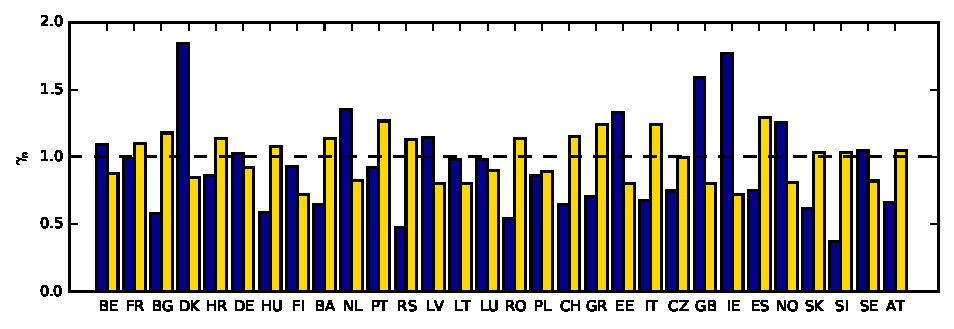
\includegraphics[width = \chromowidth, center]{beta=1}
    \caption{Examples of $\beta$ layouts for $\beta = 1$.}
    \label{fig:betaExamples}
  \end{subfigure}
  \begin{subfigure}{2\columnwidth}
    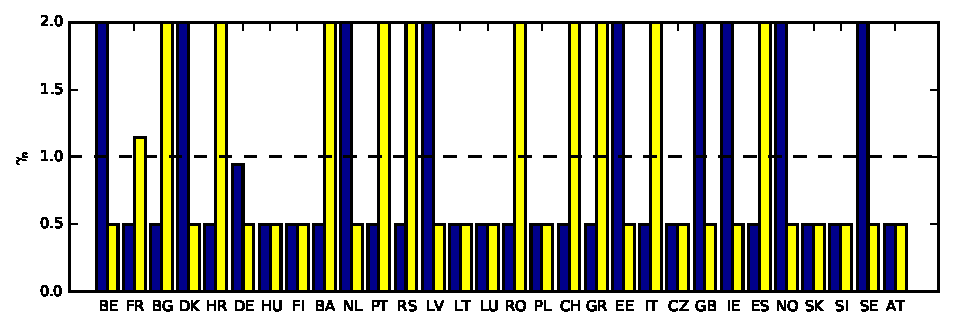
\includegraphics[width = \chromowidth, center]{k=2cfMax}
    \caption{Examples of CF layouts constrained by K = 2 .}
    \label{fig:cfMaxExamples}
  \end{subfigure}
  \caption{Examples of heuristic layouts. In each sub figure, two sets
    of bars are shown corresponding to the $\alpha_{EU} = 1$ and $0$
    layouts.}
  \label{fig:examples}
\end{figure*}

\subsection{Optimised layouts}
\label{sec:optimized-layouts}

In this subsection the full optimisation of the layouts is considered,
with the objective to minimise the \gls{lcoe} with respect to the 60
variables $\gamma_{1}, ..., \gamma_{N}, \alpha_{1}, ..., \alpha_{N}$
for the $N=30$ countries.  Given the non-linear formuation of the
problem in sections \ref{sec:network} and \ref{sec:key}, a number of non-linear
optimisation algorithms were tested including the Nelder-Mead method
\cite{nelder}, simulated annealing \cite{sa}, genetic algorithms
\cite{ga} and cuckoo search \cite{cs}. It was found that the continous
enforcement of the normalisation criteria \cref{eq:norm} generally
decreased the performance of the tested algorithms, and for that
reason a new hybrid algorithm was developed to address this problem. While being
a classical greedy algorithm in the sense that the locally optimal
choice is always taken, the renormalisation problem was circumvented
by moving only along the axial directions. The algorithm has been
denoted Greedy Axial Search (GAS), and it is decribed in detail in
\cref{sec:greedy-axial-search}. All optimised layouts have been obtained using
the GAS routine. These layouts will be denoted `GAS layouts'. To
decrease computation time, optimisations were performed using a one
year slice of the 32 year data set. The slice was chosen as the one
that statistically resembles the complete data set the most.

% Note, tables DOES NOT belong here. Just moved for layout reasons :)
\begin{table*}[t!]
  \centering
  \caption{Componentwise \gls{lcoe} for the optimal $\beta$, CF and GAS layouts along with the
    homogeneous layout without transmission. The $K$ values are expressed through the index
    notation, e.g. $K = i$ for $\beta_{i}$. All costs are listed in \euro/MWh.}
  \label{tab:cost}
  \begin{tabular}{ccrrrrrrrrr}
    \toprule
    \textbf{Parameter} & \textbf{No transmission} & $\boldsymbol\beta\mathbf{_{1}}$ & $\mathbf{CF_{1}}$ & $\mathbf{GAS_{1}}$ & $\boldsymbol\beta\mathbf{_{2}}$ & $\mathbf{CF_{2}}$& $\mathbf{GAS_{2}}$ & $\boldsymbol\beta\mathbf{_{3}}$ & $\mathbf{CF_{3}}$ & $\mathbf{GAS_{3}}$ \\
    \midrule
    $\mathcal{K}^{W}$ & 42.79 & 42.79 & 42.79 & 29.80 & 39.83 & 36.52 & 29.20 & 38.18 & 32.79 & 28.53 \\ % Onshore wind
    $\mathcal{K}^{S}$ & 6.91 & 6.91 & 6.91 & 10.59 & 6.75 & 6.25 & 8.24 & 6.66 & 5.92 & 6.72 \\ % Solar
    $\mathcal{K}^{B}$ & 6.92 & 4.88 & 4.88 & 5.40 & 4.89 & 4.93 & 5.19 & 4.91 & 5.00 & 5.11 \\ % Backup
    $E^{B}$ & 16.70 & 10.69 & 10.69 & 12.94 & 10.68 & 10.71 & 11.54 & 10.71 & 10.84 & 10.89 \\ % Fuel
    $\mathcal{K}^{T}$ & 0.00 & 2.95 & 2.95 & 3.43 & 3.12 & 4.09 & 4.54 & 3.42 & 5.26 & 5.65 \\ % Transmission
    \midrule
    Total & 73.32 & 68.22 & 68.22 & 62.16 & 65.27 & 62.50 & 58.71 & 63.88 & 59.81 & 56.90 \\
    \bottomrule
  \end{tabular}
\end{table*}

\subsection{LCOE transmission approximation}
\label{sec:approximate-lcoe}

There is a trade-off between the LCOE and the amount of transmission
capacity $\mathcal{K}^{T}$ in the system. This trade-off is illustrated in
\cref{fig:transmission-lcoe} for the homogeneous layout at
$\alpha_{EU} = 0.84$ by taking the full $\mathcal{K}^{T}$ and scaling
it down uniformly by a factor $\zeta$.

Because extreme events in terms of backup capacity (all countries have
a large energy deficit) and transmission capacity (some countries have
an energy deficit while others have excess generation) are generally
not overlapping, scaling down the $\mathcal{K}^{T}$ initially tends to
lower the \gls{lcoe} since the backup capacity $\mathcal{K}^{B}$ is
not increased accordingly.


\begin{figure}[h!]
  \centering
  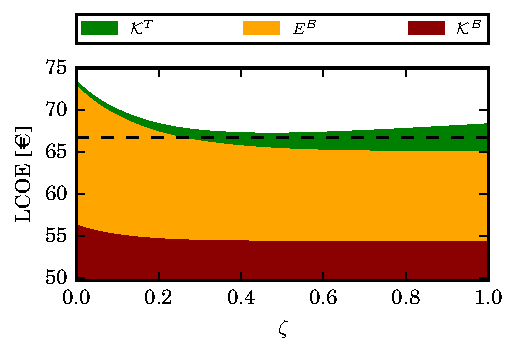
\includegraphics[width = \columnwidth]{constrainedSync-new}
  \caption{Non-\gls{vres} components of the \gls{lcoe} for different
    values of $\zeta$. The constant \gls{vres} part (omitted) consists of
    42.8\euro/MWh for wind and 6.9\euro/MWh for solar. The dashed line indicates the approximated
    \gls{lcoe} (see text). The calculations were performed using a
    homogeneous layout with $\alpha_{EU} = 0.84$ (cost optimal mix)
    and the synchronised export scheme.}
  % Solar cost is 6.91, wind cost is 42.79 (combined is 49.70)
  \label{fig:transmission-lcoe}
\end{figure}

However, if the transmission capacity is increased too far towards
$\zeta=0$, the \gls{lcoe} starts to rise again, showing the benefit of a transmission grid
\cite{Rodriguez2013}.
The cost optimal value of $\zeta$
depends of the electricity system being analysed and on the specific \gls{lcoe} definition (in
the present case the optimum is around $\zeta= 0.5$).
Obtaining the lowest possible \gls{lcoe} would thus require system individual optimisation. To
avoid the additional complexity associated with such an optimisation and to define the
\gls{lcoe} function in a consistent way, the \gls{lcoe} will consistently be calculated using
the synchronised export scheme at $\zeta=1$,
but with only 50\% of the $\mathcal{K}^{T}$
cost. The approximation is shown as a dashed line in \cref{fig:transmission-lcoe}. While the
transmission approximation is not perfect, the inaccuracy associated with the approximation is small
compared to the uncertainty of the cost estimates. The inaccuracy is quantified in the next section.

\section{Results}
\label{sec:results}

\subsection{Dependence of results on wind-solar mix}

An overview of the key parameters for each of the capacity layouts
with varying $\alpha_{EU}$ and fixed $\gamma_{EU} = 1 $
is shown in \cref{fig:overview}. For
backup energy and backup capacity, the optimal mix is around
$\alpha_{EU} = 0.9$, which is slightly higher than the values found by
\cite{Heide2010,Heide2011}.
% It does NOT make sense to say that the backup optimal mix for the
% GAS layout is 0.8; we only have a point, not a curve!
The difference can be attributed to differences between the \gls{rea} data used in this paper
and the \gls{iset} (former ISET) data \cite{iset} used by \cite{Heide2010,Heide2011}. For
transmission capacity, the curves are quite similar for the $\beta$
layouts with a minimum around $\alpha_{EU} = 0.5$.
For the CF layouts a larger increase in $\mathcal{K}^{T}$
is observed as K is increased. This observation is in qualitative agreement with intuition
since the CF layouts are generally more extreme than the $\beta$
layouts. % (see e.g. \cref{fig:optLayouts}).

%, indicating a high share of
%solar PV. While the wind correlation length is around $\approx$ 1000
%km \cite{Widen2011} and thus smaller than Europe, the occurrence of
%sun light is highly correlated for the European countries.
%\cite{Timo}.
%Therefore, a high wind share causes more power to flow
%between the countries.

The main parameter of interest, the \gls{lcoe}, has a maximum at
$\alpha_{EU} = 0$. For the $\beta$ and CF layouts it drops steadily as
$\alpha_{EU}$ is increased until around $\alpha_{EU} = 0.84$ where the minimum
is located. The GAS optimised layouts are also to be found in the wind
dominated region, but their $\alpha$ values are generally lower. The high
cost at $\alpha_{EU} = 0$ is caused by a combination of high backup
energy/capacity costs and the fact that the CF of solar is generally
lower than for onshore wind. The cost of producing one unit of energy
is thus higher for solar than for onshore wind even though the
\gls{CapEx} is lower for solar.


%From the
%comparison it is clear that the approximation is generally
%underestimating the \gls{lcoe}, and the approximation becomes worse as K is
%increased. At $K=2$ the approximated \gls{lcoe} is off by 1.3\%.

\begin{figure*}[t!]
  \centering
  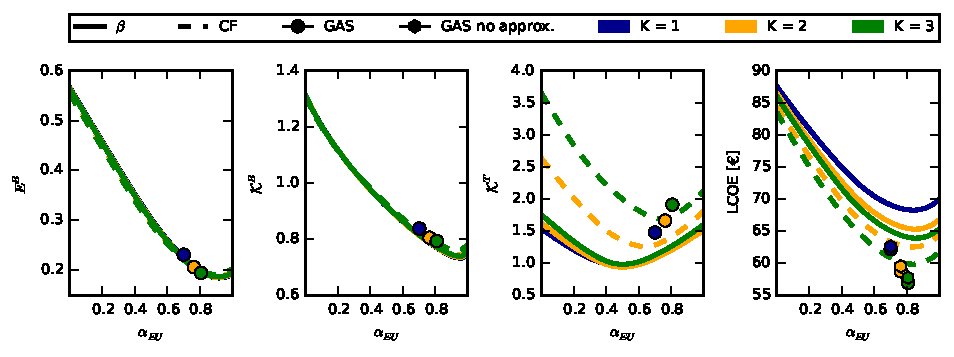
\includegraphics[width = 2\columnwidth]{dataSync-new}
  \caption{Overview of the key parameters and the associated \gls{lcoe} as a
    function of $\alpha_{EU}$. The $\beta$ %(solid line)
    and CF %(dashed line)
    layouts are shown as solid and dashed lines respectively. The GAS
    layouts are plotted as dots. Different constraints are shown: K =
    1 (blue), 2 (yellow) and 3 (green).}
  \label{fig:overview}
\end{figure*}

\subsection{Cost comparison of different layouts}

The componentwise costs for the $\alpha$-optimal $\beta$, CF and GAS layouts
are given in \cref{tab:cost} and graphed in \cref{fig:cost}.

If the total \gls{lcoe} is considered, there is a clear trend of cost
reduction as the heterogeneity parameter $K$ is increased, allowing
sites with better capacity factors to be exploited. For each
value of $K$ the cost is also reduced as the layout is optimised further
from the $\beta$ to the CF to the GAS layout. At $K=1$ the \gls{lcoe}
sinks by 9\% from the homogeneous layout at 68.2\euro/MWh to
62.2\euro/MWh in the GAS layout. At $K=3$ there is more freedom for
the GAS algorithm to optimise the heterogeneous layout and the cost
drops 11\% from 63.9\euro/MWh in the $\beta$ layout to 56.9\euro/MWh
in the GAS layout.

With regard to the costs of each component of the \gls{lcoe}, the
transmission costs are higher in the GAS layout than the heuristic
layouts due to the more heterogenous distribution of \gls{vres}, but
this is more than offset by the reduction in \gls{vres} costs, which
dominate the total costs. The reduction in \gls{vres} costs is a
direct result of the improved average capacity factors in the GAS
layout, which allow the same energy yield for lower overall
capacity. Compared to the transmission and \gls{vres} costs, the
backup costs remain relatively constant.



One reason that the GAS optimisation might have been better than the
heuristic layouts is that the GAS algorithm sees not just the capacity
factors at each site, like the heuristic layouts, but also the
geographical variation of the temporal generation pattern, which the
GAS algorithm can exploit to shape the \gls{vres} generation pattern
to the load. However if this was the reason, the backup generation
costs would have decreased from the heuristic to the GAS layout, which
they do not; in fact the backup costs rise very slightly. This
suggests that the GAS optimisation's success really lies with the freer
exploitation of capacity factors.


Compared to the $\beta$
and CF layouts, the GAS layouts include a slightly larger solar component. The magnitude of the
solar component for the GAS layouts drops with increasing K value. As the heterogeneity
constraints are loosened wind becomes more favourable since it becomes possible to allocate
more resources to the sites with a very high CF. A similar effect is present for solar, but it
is less dominant since the difference between the higest and lowest CF for solar (0.20, Spain
vs. 0.11, Finland) is much smaller than for wind (0.37, Denmark vs. 0.07, Slovenia).

\begin{figure}[h!]
  \centering
  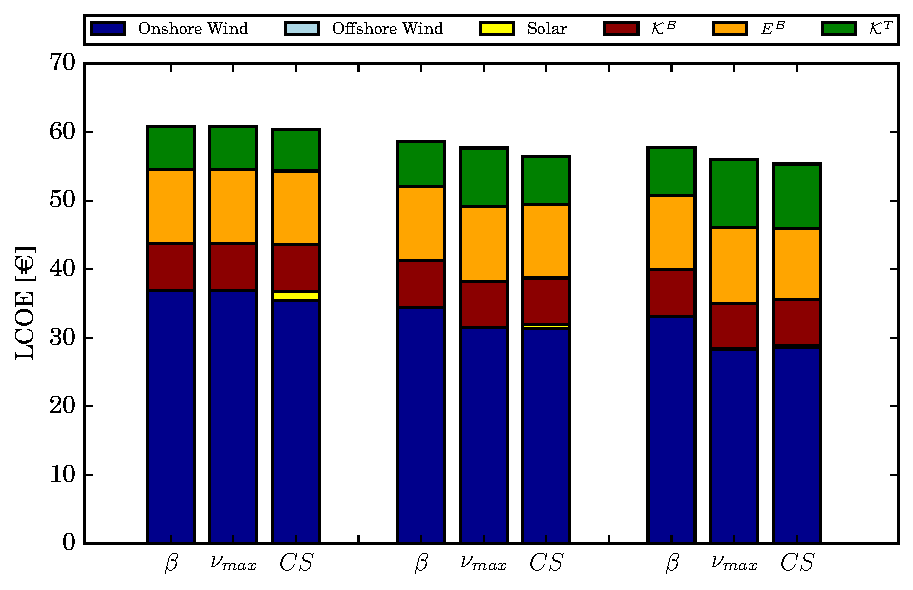
\includegraphics[width = \columnwidth]{costVE50}
  \caption{Componentwise \gls{lcoe} for the optimal $\beta$, CF and GAS layouts
    for K = 1 (left), 2 (middle) and 3 (right). The unlabelled bar
    represents the homogeneous layout without transmission.}
  \label{fig:cost}
\end{figure}



\subsection{Distribution of capacity layouts}

In this section the geographical distribution of wind and solar capacities is examined.
The $\beta$
and CF layouts for $K=2$
are compared to the homogeneous layout in \cref{fig:k=2layouts} while the GAS layouts for $K=1,2,3$ are shown
in \cref{fig:optLayouts}. %Note that for $K=1$, the $\beta$ and the CF layouts are both equal to
%the homogeneous layout.

From the two heuristic layouts shown in \cref{fig:k=2layouts} it is
clear that the CF layout achieves a much greater degree of
heterogeneity than the $\beta$ layout, whose heterogeneity is limited
by the first country to hit the $K=2$ boundary (in this case Slovenia
at $\gamma_n = 1/2$). This is reflected in the CF layout's
lower \gls{lcoe}.  In fact the CF layout is not far from the GAS
layout for $K=2$ in \cref{fig:optLayouts}: in both layouts there
is a predominance of wind in Denmark, the Netherlands, Great Britain,
Ireland and Norway.

As the heterogeneity parameter $K$ is increased for the GAS layouts,
wind dominates in terms of energy. At $K=2$ and $K=3$ it is
interesting to note that all the countries are either completely solar
or completely wind dominated (with the only exception of Lithuania for
$K=3$, which is mostly wind). This choice appears to be entirely correlated with which
\gls{vres} technology has the higher capacity factor in each country (see
\cref{tab:capacity-factors} for the capacity factors; the only
exception is Croatia, where the capacity factors are anyway very close
together). This confirms that the GAS algorithm is largely optimising
by capacity factor.


\subsection{Transmission capacities}

As seen in \cref{fig:cost}, the cost of transmission increases with increasing
heterogeneity. To quantify what happens, the link usage for the homogeneous layout and the GAS
layout for K = 2 is visualised in \cref{fig:links}. Comparing \cref{fig:links-homo} and
\cref{fig:links-k2} it is clear that the flow does not increase homogeneously across the
network. The primary increase is on links connecting countries with severe excess generation,
e.g. Great Britain, Ireland, the Netherlands, Norway and Denmark. %(see \cref{fig:optLayouts}).
However, additional flows are also induced on links connected to Germany and France, which act
as transit countries. The capacity of links connecting south and central European countries
remains practically unchanged.

\begin{figure*}[p!]
  \centering
  \begin{subfigure}{2\columnwidth}
    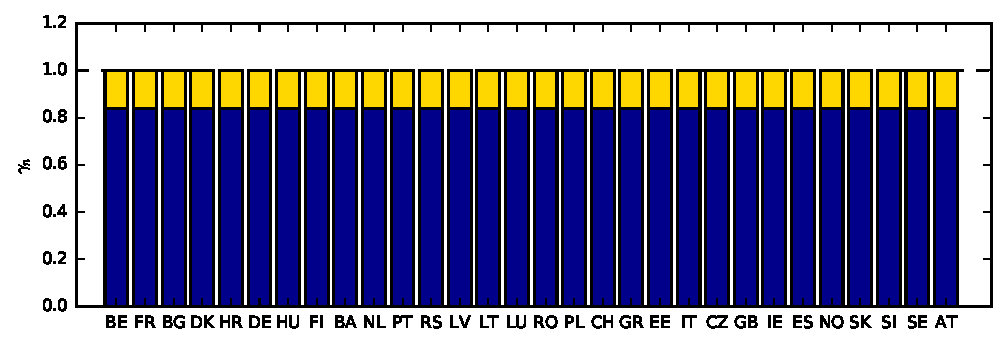
\includegraphics[width = \chromowidth, center]{chromosome_homogeneous}
    \caption{Homogeneous layout.}
    \label{fig:betaOpt}
  \end{subfigure}
  \begin{subfigure}{2\columnwidth}
    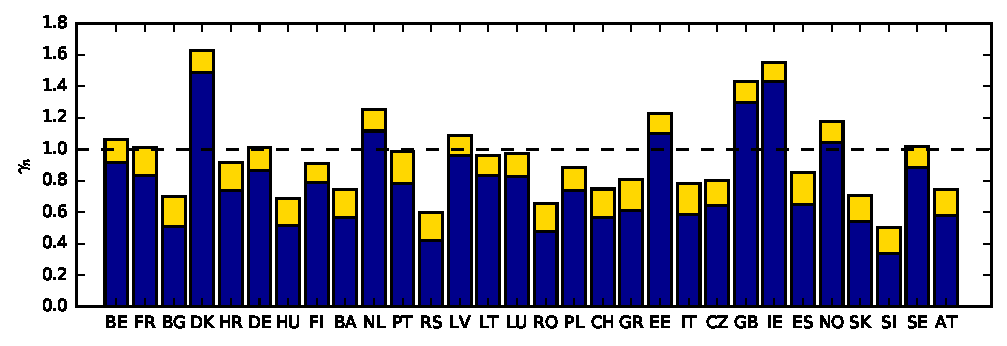
\includegraphics[width = \chromowidth, center]{chromosome_k=2beta}
    \caption{$\beta$ layout constrained by $K = 2$.}
    \label{fig:cfMaxOpt}
  \end{subfigure}
  \begin{subfigure}{2\columnwidth}
    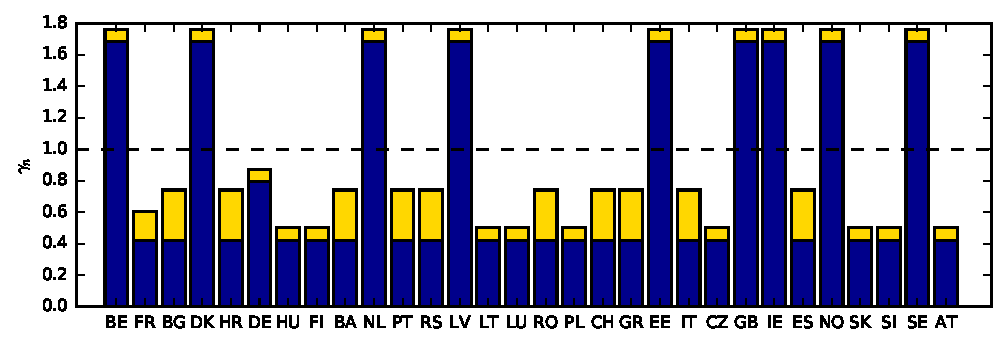
\includegraphics[width = \chromowidth, center]{chromosome_k=2cfMax}
    \caption{CF layout constrained by $K = 2$.}
    \label{fig:agdOpt}
  \end{subfigure}
  \caption{Comparison of the homogeneous layout (a) with the $\beta$
    and CF layouts constrained by $K = 2$ (b, c). }
  \label{fig:k=2layouts}
\end{figure*}

\begin{figure*}[p!]
  \centering
  \begin{subfigure}{2\columnwidth}
    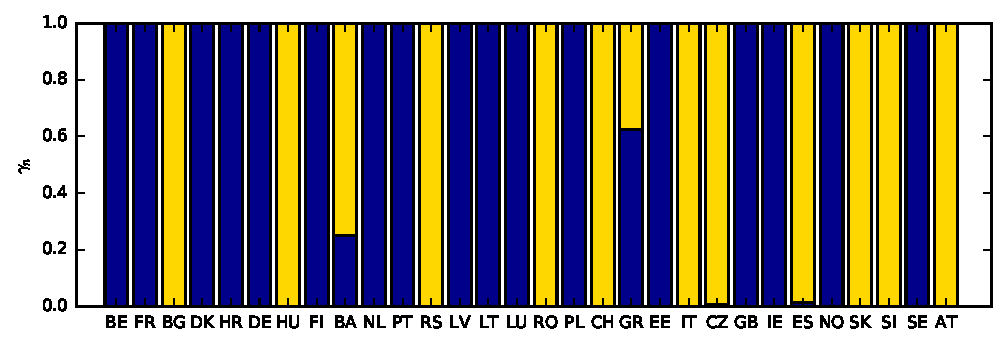
\includegraphics[width = \chromowidth, center]{chromosome_k=1gas}
    \caption{GAS layout constrained by K = 1.}
    \label{fig:betaOpt}
  \end{subfigure}
  \begin{subfigure}{2\columnwidth}
    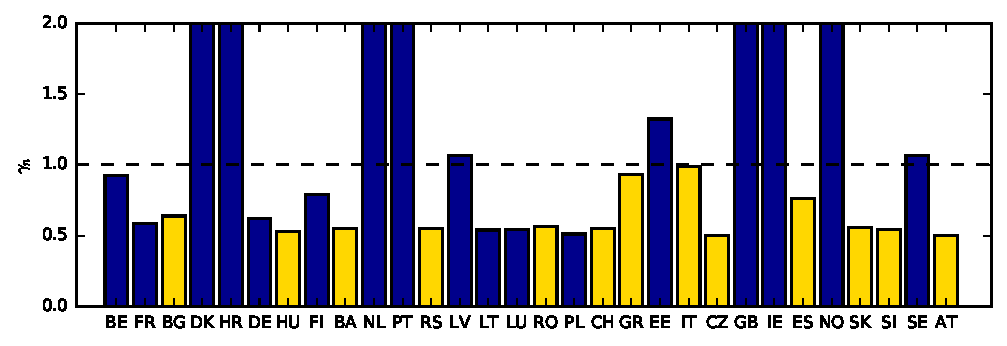
\includegraphics[width = \chromowidth, center]{chromosome_k=2gas}
    \caption{GAS layout constrained by K = 2.}
    \label{fig:cfMaxOpt}
  \end{subfigure}
  \begin{subfigure}{2\columnwidth}
    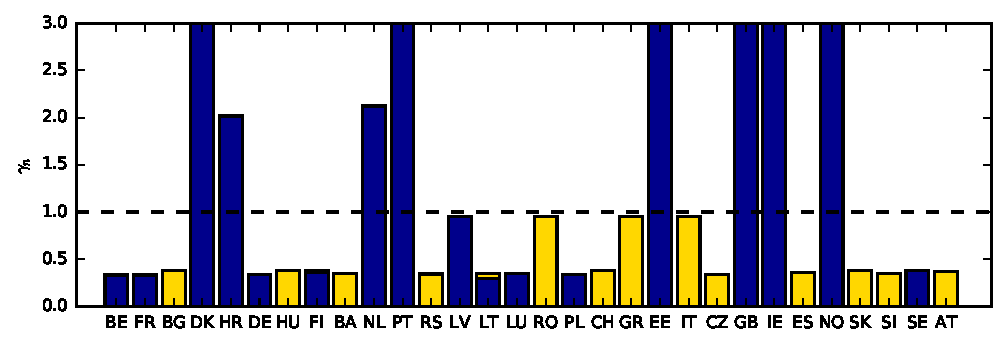
\includegraphics[width = \chromowidth, center]{chromosome_k=3gas}
    \caption{GAS layout constrained by K = 3.}
    \label{fig:agdOpt}
  \end{subfigure}
  \caption{GAS optimised layouts for different k values.}
  \label{fig:optLayouts}
\end{figure*}





\begin{figure*}[t!]
  \centering
  \begin{subfigure}{1\columnwidth}
    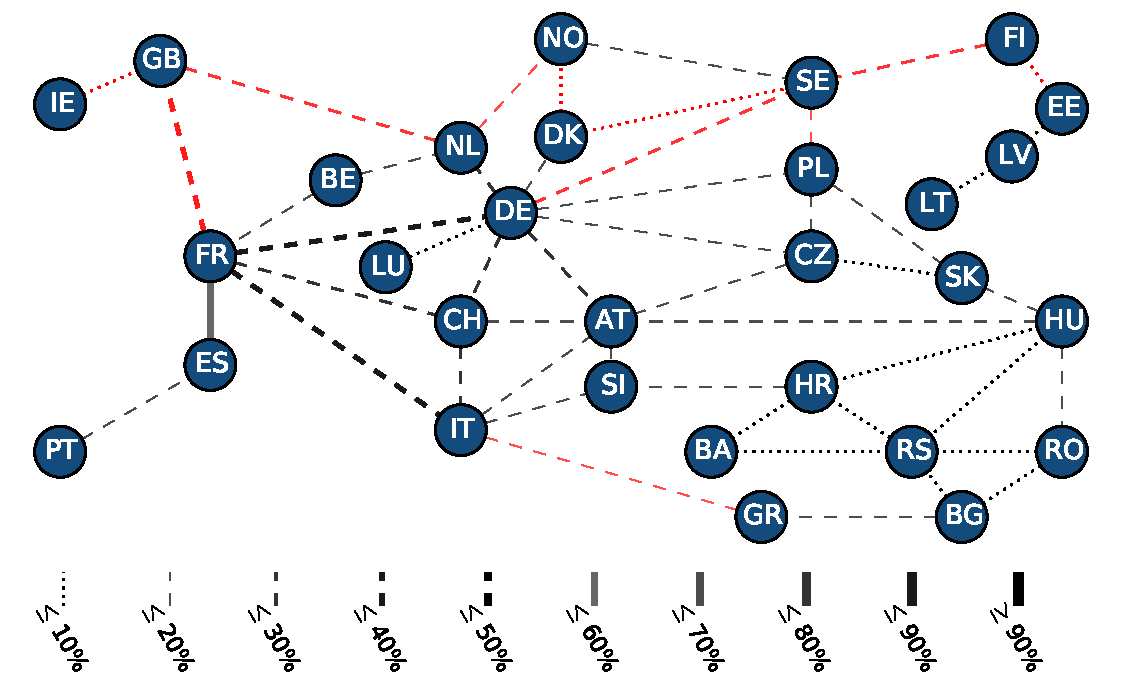
\includegraphics[width = \columnwidth, center]{links-homogeneous}
    \caption{Link usage for the homogeneous layout.}
    \label{fig:links-homo}
  \end{subfigure}
  \begin{subfigure}{1\columnwidth}
    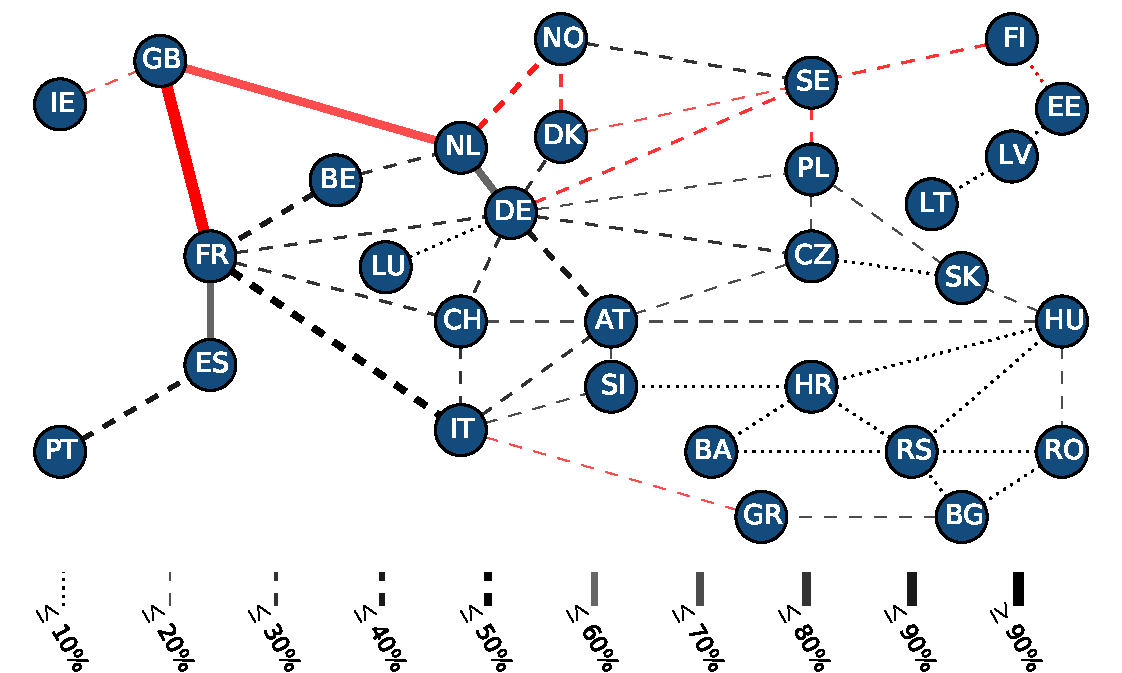
\includegraphics[width = \columnwidth, center]{links-gas-k=2}
    \caption{Link usage for the GAS layout constrained by K = 2.}
    \label{fig:links-k2}
  \end{subfigure}
  % The capacities shown are NOT scaled by any (beta) fraction.
  \caption{Overview of link usage. AC links are shown in black while
    HVDC links are shown in red. Link capacities are calculated as per
    \cref{eq:link-cap} and indicated relative to the highest flow (103 GW
    between Great Britain and France in \cref{fig:links-k2}).}
  \label{fig:links}
\end{figure*}


\subsection{Validity of transmission approximation}


To assess the validity of the \gls{lcoe} transmission approximation
proposed in \cref{sec:approximate-lcoe}, the value of $\zeta$ was
optimised to minimise the \gls{lcoe} for the values of $\gamma_n,\alpha_n$ in
the GAS layout for each value of $K$. The results are plotted in
\cref{fig:overview} as hexagons, where the optimised values
of $\zeta$  are 0.43, 0.44 and 0.45 for K = 1, 2 and 3 respectively.

From the comparison it is clear that the approximation generally works well. The \gls{lcoe} is
underestimated slightly, and the error tends to increase with $K$.
At $K=2$ the approximated \gls{lcoe} is off by 1.3\%.


\section{Sensitivity analysis}
\label{sec:sensitivity-analysis}

%\subsection{Excluding transmission in the optimization}
%\label{sec:incl-transm-optim}
%
%While the main findings include only three optimized layouts, for K =
%1, 2 and 3, numerous optimizations must be performed to allow
%convergence analysis, parameter tuning, and sensitivity analysis. In
%this case, each optimization taking more than a day is impractical.
%
%As mentioned in \cref{sec:cuckoo-search}, the computation time can be
%decreased by analysing only a subset of the 32 years of data. However,
%going below one year is not ideal as this choice would imply
%neglecting important seasonal fluctuations. Numerically, the most
%costly operation in the analysis is the quadratic optimization problem,
%\cref{eq:step1}, which is solved in each iteration to determine the
%flows. This step is not needed to determine backup properties. By
%skipping the step, it is possible to speed up the optimization by more
%than a factor of 50. Layouts obtained by optimization excluding
%transmission are shown in \cref{fig:cost-no-transmission}.
%
%\begin{figure}[h!]
%  \centering
%  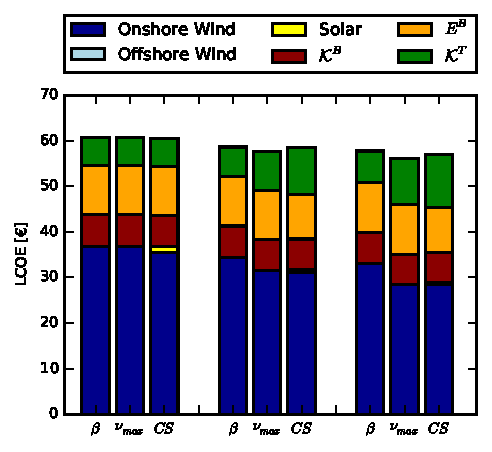
\includegraphics[width = \columnwidth]{costTransVE50}
%  \caption{Cost details for the optimal layouts for K = 1 (left), 2
%    (middle) and 3 (right) for $\beta$, CF and CS (transmission excluded).}
%  \label{fig:cost-no-transmission}
%\end{figure}
%
%It is clear that the optimization succeeds in decreasing the cost of
%all, but the transmission component. However, for K = 2 and K = 3, the
%associated increase in transmission cost is so large that the CS
%layouts end up being more expensive than the CF layouts at
%$\alpha = 1$. The difference between the CS layouts with transmission
%included/excluded is noticeable, but the CS solution obtained without
%transmission is still fairly good. For convergence analysis, parameter
%tuning, and sensitivity analysis, optimizations have been performed
%excluding transmission costs. This includes all CS solutions presented
%in this section.
%
%To illustrate how the CS solution changes when transmission is taken
%into account, the link usage for the two solutions for K = 2 is shown
%in \cref{fig:links}.
%
%\begin{figure*}[p]
%  \centering
%  \begin{subfigure}{2\columnwidth}
%    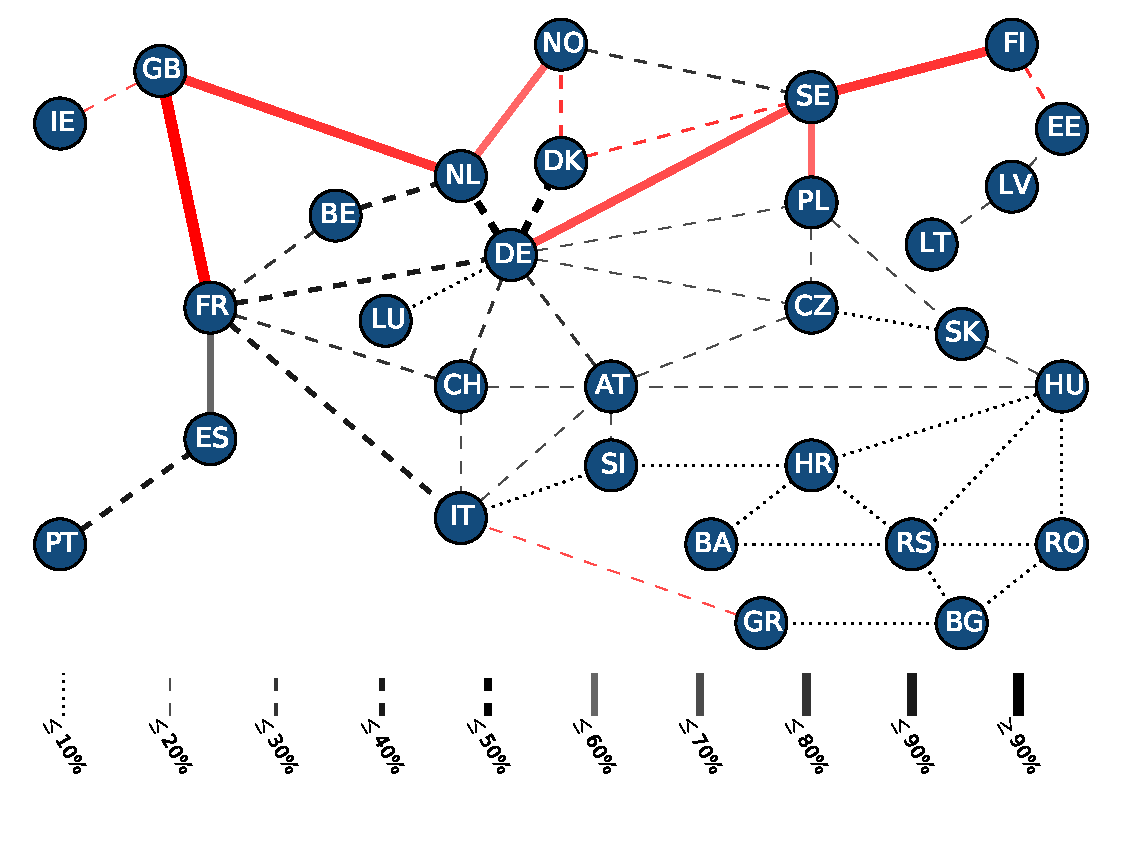
\includegraphics[width = 0.75 \columnwidth, center]{VE50cuckooK=2@defaultLINKS}
%    \caption{Link usage for the CS layout (transmission excluded)
%      constrained by K = 2.}
%    \label{fig:linksNoTrans}
%  \end{subfigure}
%  \begin{subfigure}{2\columnwidth}
%    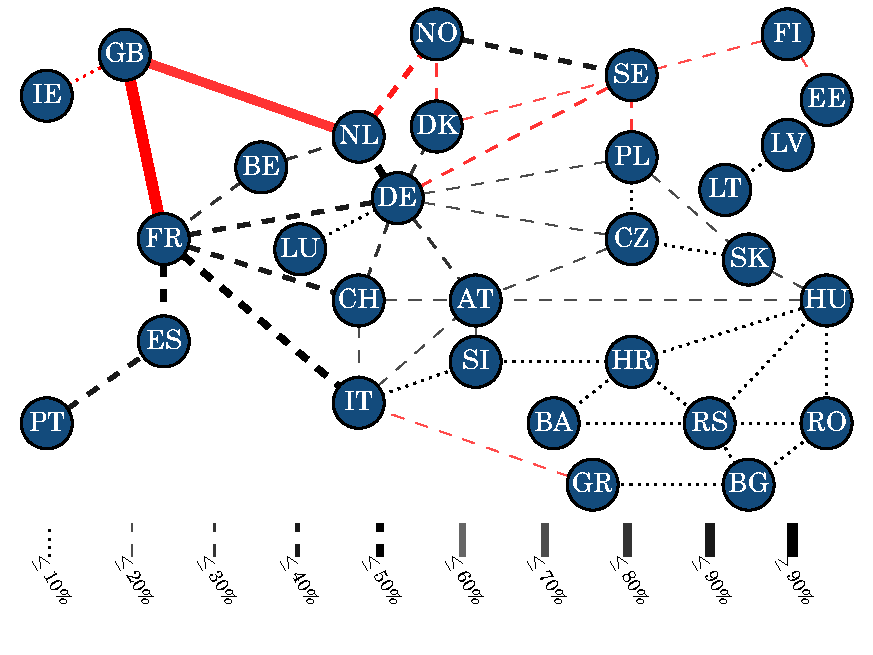
\includegraphics[width = 0.75 \columnwidth, center]{VE50cuckooK=2@TRANS10kLINKS}
%    \caption{Link usage for the CS layout (transmission included)
%      constrained by K = 2.}
%    \label{fig:linksTrans}
%  \end{subfigure}
%  \caption{Overview of link usage. AC links are shown in black while
%    HVDC links are shown in red. Link capacities are indicated
%    relative to the highest flow (74 GW between Great Britain and
%    France in \cref{fig:linksNoTrans}). As transmission costs are included in
%    the optimization, the layout is altered in a way that tends to
%    decrease the load on HVDC links. This tendency can be attributed
%    to the fact that the cost of HVDC links is significantly higher
%    than the cost of AC links. An exception is Great Britain where
%    $\nu^{W}$ is so high that the resulting low cost of wind energy
%    outweighs the cost of the HVDC connections.}
%  \label{fig:links}
%\end{figure*}
%
%From \cref{fig:links} we see that in the CS layout obtained with
%transmission included, the resources have been reallocated in such a
%way that the link usage is decreased. In particular, the load on HVDC
%links (shown in red) is lower. Since the cost of HVDC links is
%significantly higher than the cost of AC links, it makes perfect sense
%that the load on these links has been decreased the most.

\subsection{Reduced solar cost}
\label{sec:reduced-solar-cost}

For the $\beta$ as well as the CF layouts, the optimal mix is around
$\alpha_{EU}=0.84$. As mentioned previously, wind domination is partly a
consequence of the higher cost of energy generation for solar PV
compared to onshore wind. The cost of solar has dropped rapidly in the
recent years and this tendency might very well continue. To shed some
light on the consequences of further price reductions, the sensitivity
of the optimal mix to reductions in the solar cost has been
examined. \Cref{fig:red-solar} illustrates the change in \gls{lcoe} for the
GAS optimised layouts when the solar cost is reduced by 25\%, 50\% and
75\% respectively. The 0\% scenario is included as a reference.

\begin{figure}[h!]
  \centering
  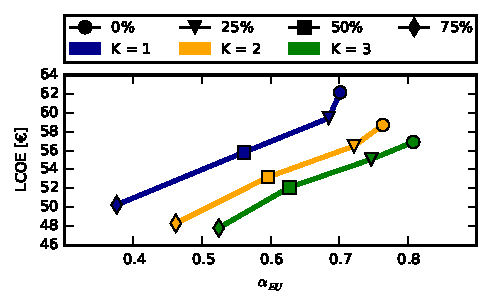
\includegraphics[width = \columnwidth]{solarAnalysis-new}
  \caption{\gls{lcoe} of the GAS optimised layouts when the solar cost is
    reduced by 25\% (triangle), 50\% (square) and 75\% (diamond). The
    0\% scenario (circle) is included as a reference. Different
    constraints are shown: K = 1 (blue), 2 (yellow) and 3 (green).}
  \label{fig:red-solar}
\end{figure}

A reduction of the solar cost by 25\% does not change the picture
much. The optimal mix is shifted from above 0.75 to below 0.75 and the
\gls{lcoe} drops by around 2\euro{} (cost comparison numbers are calculated
for the GAS layouts at K = 2).  As the solar cost is reduced by 50\%
the cost at $\alpha_{EU} = 0$ (pure solar) becomes comparable to the
cost at $\alpha_{EU} = 1$ (pure wind). The optimal mix drops to around
0.6 and the \gls{lcoe} is reduced by almost 6\euro{} compared to the
reference scenario. Reducing the cost of solar by 75\%, solar becomes
much cheaper than wind, and the optimal mix is shifted below
$\alpha_{EU} = 0.5$ indicating solar domination. Compared to the
reference scenario, the \gls{lcoe} dropped by more than 10\euro. However, it
should be noted that such large cost reductions for PV may not be
plausible: much of the recent cost reduction  has come from reduced material costs; the remaining costs come from the installation, where it is not so easy to economise.

\begin{figure*}[t!]
  \centering
  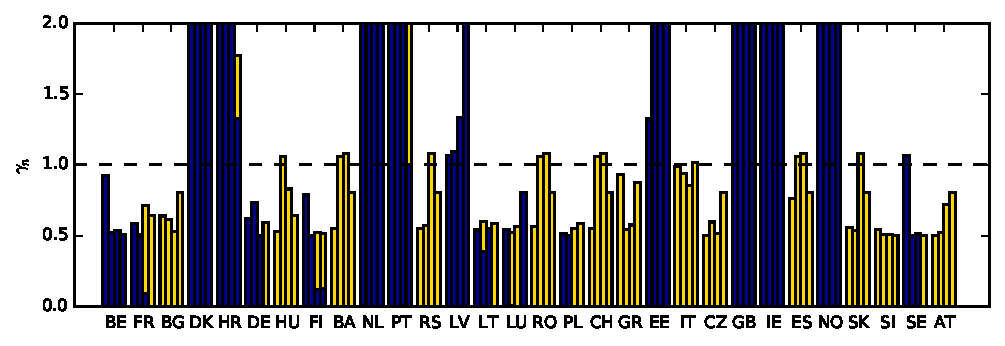
\includegraphics[width = 2\columnwidth, center]{solarAnalysis-layouts}
  \caption{GAS optimised layouts constrained by K = 2 for a solar cost
    reduction of (from left to right) 0\% (reference), 25\%, 50\% and
    75\%.}
  \label{fig:layout-offshore}
\end{figure*}

% The
%exact optimal mix $\alpha$ values are listed in \cref{tab:solar-alpha}.

% DROP VALUES: 2.23 at 25\%, 5.51 at 50\%, 10.41 at 75\% (comared to
% reference scennario, GAS optimised layouts at K = 2.

% \begin{table}[h!]
%   \centering
%   \caption{Alpha values for optimal layouts for different scalings of
%     the solar cost.}
%   \label{tab:solar-alpha}
%   \begin{subtable}{\columnwidth}
%     \centering
%     \caption{Cost reductions by a factor of 2.}
%     \begin{tabular}[h!]{l c c c}\toprule
%       & K = 1 & K = 2 & K = 3 \\ \midrule
%       $\beta$ & 0.87 & 0.87 & 0.93 \\
%       CF & 0.87 & 0.87 & 0.87 \\
%       GAS & 0.80 & 0.87 & 0.90 \\ \bottomrule
%     \end{tabular}
%     \vspace{10pt}
%   \end{subtable}
%   \begin{subtable}{\columnwidth}
%     \centering
%     \caption{Cost reductions by a factor of 4.}
%   \begin{tabular}[h!]{l c c c}\toprule
%     & K = 1 & K = 2 & K = 3 \\ \midrule
%     $\beta$ & 0.67 & 0.67 & 0.67 \\
%     CF & 0.67 & 0.67 & 0.73 \\
%     GAS & 0.69 & 0.75 & 0.78 \\ \bottomrule
%   \end{tabular}
% \end{subtable}
% \end{table}

\subsection{Offshore wind}
\label{sec:offshore-wind}

So far, wind has been assumed to be onshore only. By January 2014, the
total European onshore wind capacity was 120.8GW, while the offshore
capacity was 8.0GW \cite{EWEA}. %While these numbers confirm the
%onshore only assumption to be reasonable,
The increasing share of offshore wind raises the question, how the
\gls{lcoe} will be affected by the introduction of an offshore
component. The immediate expectation would be a significant increase
in the \gls{lcoe}, since the expenditures for offshore wind are more than
100\% higher than for onshore wind due to foundation expenses and
increased maintenance costs. On the other hand the capacity factors
for offshore sites are generally higher than for onshore sites.

It would be possible to introduce offshore wind on equal footing with
onshore wind and solar PV. However, since offshore wind is much more
expensive, an optimised layout would pose a 0\% offshore component,
which is not an interesting nor surprising result. Instead, a fixed
offshore component is introduced by splitting the wind component into
an onshore $\gamma^{W}$ and an offshore $\gamma^{\tilde{W}}$ component,

\begin{equation}
  \label{eq:11}
  \gamma^{W} \to \gamma^{\text{W}} + \gamma^{\text{$\tilde{W}$}},
\end{equation}

for countries with suitable offshore regions. In practice these are
the North Sea countries (Denmark, Germany, Great Britain, Ireland, the
Netherlands, France, Belgium, Norway and Sweden). Other countries
retain onshore wind only. The magnitude of the offshore component is
defined by requiring that the offshore wind power generation accounts
for a fixed share of the total wind power generation. %,
%
%\begin{equation}
%  \label{eq:12}
%  \text{offshore share = }\frac{\gamma^{\tilde{W}}}{\gamma^{W}}.
%\end{equation}
%
Cost details for optimised layouts with fixed offshore shares of 25\%
and 50\% are shown in \cref{fig:cost-offshore}. The 0\% scenario is
included as a reference.

\begin{figure}[h!]
  \centering
  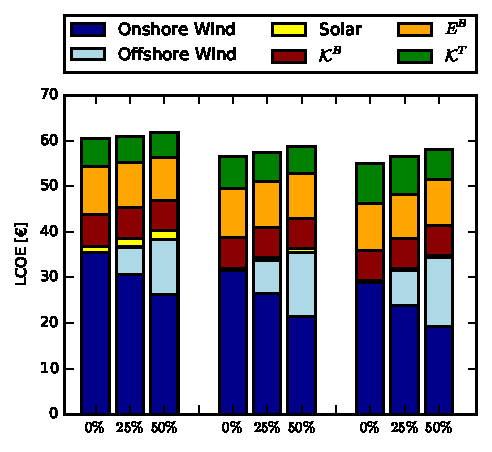
\includegraphics[width = \columnwidth]{costOffshoreVE50}
  \caption{Cost details for the GAS optimal layouts for K = 1 (left),
    2 (middle) and 3 (right) for offshore shares of 0\%, 25\% and 50\%.}
  \label{fig:cost-offshore}
\end{figure}

From \cref{fig:cost-offshore} it is clear that the introduction of an
offshore component increases the \gls{lcoe}. However, the increase in \gls{lcoe}
is not dramatic. While the cost of wind increases
significantly, the cost of backup and transmission decreases
slightly. The decrease is a consequence of the difference in the
temporal generation pattern from onshore to offshore wind. In some
time steps the onshore generation is low while the offshore generation
is high. The introduction of an offshore component thus tends to
smooth out the wind generation time series. %As a side effect, opposite
%of what one might have expected, solar becomes less favourable as
%illustrated by \cref{fig:cost-offshore}.
The GAS optimised layouts for an offshore share of 50\% are shown in
\cref{fig:layout-offshore}.

\begin{figure*}[t!]
  \centering
  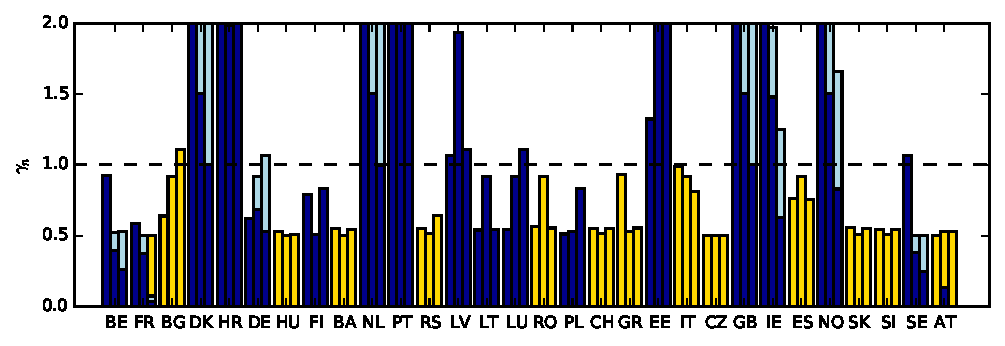
\includegraphics[width = 2\columnwidth, center]{offshoreLayouts-new}
  \caption{GAS optimised layouts constrained by K = 2 for an offshore
    share of (from left to right) 0\% (reference), 25\% and 50\%.} % for
    %the North Sea countries.}
  \label{fig:layout-offshore}
\end{figure*}

%*************************************************************************
\section{Discussion and conclusions}
\label{sec:four}
%*************************************************************************

The cost-optimal distribution of \gls{vres} around Europe has been
investigated for the case where the mean \gls{vres} generation equals the
mean load ($\gamma_{EU} = 1$). It was found that although the costs of
backup generation and transmission are significant, the main costs are
associated with the \gls{vres} capacities. The \gls{vres} capacity costs can be
lowered by allocating more resources to countries with high capacity
factors and by preferring onshore wind over solar PV. Allowing each
country to install \gls{vres} capacities covering a minimum of 50\% and a
maximum of 200\% of their mean load, the \gls{lcoe} can be lowered by more
than 8\% by choosing the heuristic CF layout which maximises the
overall capacity factor. An additional 6\% reduction of the \gls{lcoe} was
achieved by explicit optimisation, whose final layout was close to the heuristic CF layout based only on capacity factors. This cost reduction can be
attributed to the general tendency for the heterogeneous layouts to
shift wind capacities towards the North Sea countries. Since the wind
resource quality is better than for the central and southern
countries, this reallocation results in lower costs.

In the past onshore wind has been the predominant \gls{vres} and the
cost-optimal mixes presented here are also dominated by onshore wind,
based on current cost projections.  However, the cost of solar PV has
dropped more rapidly than expected in recent years, and solar PV has
already reached grid parity in some markets \cite{solarGridParity}. If
this decreasing price trajectory continues much longer, the cost
optimal mix may end up around $\alpha_{EU} = 0.6$,
indicating almost equal amounts of wind and solar in the energy mix.

% A cost reduction of 7\% compared to the homogeneously might seem
% minor, but since the cost of a ?? is on the ??? scale, 7\% is
% actually a very significant cost reduction.

%The cost reduction is a strong argument for a heterogeneous
%layout. However, the realisation might be a political challenge. Since
%the optimal placing of resources was derived from a system
%perspective, a realisation would require full collaboration from all
%countries. Countries with low capacity factors would no longer be self
%sufficient, and they would be forced to invest in foreign
%capacities. Convincing countries to let go of the independence of
%their electricity system and to move capital abroad might require some
%political effort. On the other hand, locating sufficient sites for
%onshore wind in the North Sea countries might very well pose a
%challenge too.

% The cost optimal layouts considered in the main analysis are almost
% exclusively based on onshore wind. The reason is that onshore wind is
% significantly cheaper than solar, partly due to lower capital
% expenses, partly due to higher capacity factor. It was found that the
% cost of solar must decrease by a factor of $\approx$ 2 for a
% significant solar component to become profitable. Besides lowering the
% capital expenses, the solar cost could also be lowered by increasing
% the capacity factor. Based on data from \cite{REA}, the capacity factor can
% be increased by $\approx$ 40\% by applying dual axis tracking compared
% to the fixed position installation assumed in
% \cref{tab:capacity-factors}. In addition, studies on increasing the
% energy conversion efficiency are still being conducted.

The main analysis considered onshore wind only, but the effect of
introducing an offshore component was also discussed. Although
capacity factors offshore are higher than onshore and the temporal
generation pattern is more stable, these advantages are offset by the
higher costs arising from expensive offshore foundations and increased
maintenance costs. However, offshore wind has several other benefits:
the opposition from the public is usually lower than for onshore wind,
and the potential for expansion larger. When feasible onshore sites
have been exhausted, offshore wind might present the best alternative.

% There is A LOT of potential for the outlook; the sky is the limit...

There are several avenues for further investigations. The cost assumption for the backup generation is based on the
worst-case scenario that all backup is provided by gas turbines. In
reality, up to 17\% of Europe's electricity supply is already provided
by hydroelectric plants, most of which are flexible, some of which
have storage capacity and all of which produce electricity at very low
marginal cost. Incorporating hydroelectricity in the modelling would
reduce the \gls{lcoe} further.

In addition, a full assessment of the geographical resource potentials
in each country for each \gls{vres} technology would allow further
heterogeneity beyond the $K=2,3$ limits considered here, which would
also result in a lower \gls{lcoe}. Similarly an increase in the
spatial resolution of the model would allow more fine-tuned allocation
of renewables to sites with the highest capacity factors, resulting in a yet lower \gls{lcoe}.

An unequal distribution of renewable energy generation raises the
question of who should pay for the generation and transmission
assets. Recent work on the allocation of network flows to
users in highly renewable networks \cite{Brown2014,Tranberg} may
provide the basis for an equitable distribution of the costs of a
highly heterogeneous system.



%Even moderate amounts of
%storage can decrease the backup needs significantly[REF].

%For small amounts of storage, the optimal mix will most likely be
%lowered, as the day-night cycle solar makes it

% An exploration of layouts of \gls{vres} capacities over Europe shows that
% heterogeneous layouts are capable of significantly increasing the
% overall capacity factor $\nu_\text{EU}$ of renewables, while reducing
% the standard deviation $\sigma_\text{EU}$ of their generation. By scaling
% the regional penetration of renewables according to countries'
% capacity factors, we produce a heterogeneous mixture that favours
% installation primarily in countries around the North Sea, since wind
% is preferable to solar to increase $\nu_\text{EU}$ and reduce
% $\sigma_\text{EU}$. These improvements lead to an overall reduction in
% the cost of electricity generated by the system.

% Optimal layout theory helps analyse the space of heterogeneous
% layouts. By mixing wind- and solar-only layouts that lie along the
% Pareto front, we find configurations that further reduce the risk
% ($\sigma_\text{EU}$) while increasing the return
% ($\nu_\text{EU}$). However, the increased heterogeneity that these
% systems propose imply such an increase in transmission that the
% total system cost is greater than a system scaling by regional
% capacity factors. A genetic algorithm is the used to further explore
% heterogeneous layouts. With the explicit aim of reducing system
% costs, the genetic algorithm finds a very heterogeneous system that
% is nonetheless able to significantly reduce system costs, mainly
% through a marked increase in the European capacity factor
% $\nu_\text{EU}$.

% nu is defined by country-wide avetage, thats why spainis os bad,
% ahigher reoltuon might show interesting results

%\FloatBarrier

% *************************************************
\section*{Bibliography}
% *************************************************

\bibliographystyle{unsrt}%model3-num-names}
\bibliography{references}

\appendix

\renewcommand{\thesection}{Appendix \Roman{section}}
\section{Greedy Axial Search}
\label{sec:greedy-axial-search}

When a solution is renormalised, all $\gamma$ values are scaled either up
or down. Therefore, it is possible that some $\gamma$ values end up outside
the boundaries. Applying the box method and doing another rescaling
would normally cause an infinite loop, but if the troublesome $\gamma$
values are fixed at the boundary and the rescaling is only applied to
the remaining free $\gamma$ values, the infinite loop is avoided. In
general this approach is problematic since it can change the direction
of the search. However, in one particular case, that does not
matter. Consider a step up/down in $\gamma$ along axis $i$. In this case
all other $\gamma$ values are scaled down/up. Keeping $\gamma_{i}$ fixed while
applying the renormalisation procedure as described above, the
feasibility of moving up/down \textit{along axis $i$} can be
determined. This is the underlying principle of \gls{gas}.

As any greedy algorithm, the \gls{gas} algorithm works by taking the
locally optimal choice. Hence the feasibility for each direction is
evaluated, but only the best choice is accepted. This process is
repeated until a convergence criteria is fulfilled. At this point the
step size is reduced and the iterative optimisation procedure repeated
until the step size drops below some tolerance. The algorithm
structure is sketched in \cref{gasAlgo}.

The \textit{StepUp} and \textit{StepDown} subroutines generate new
solutions by stepping a solution (first argument) up/down along
dimension $i$ (second argument) with some step size (third argument)
after which the solution is renormalized as described above. Compared
to \cref{gasAlgo} a few tricks have been implemented to improve
performance (e.g. if the step up along dimension $i$ turned out to be
favourable, the step down solution is not evaluated). Performance
tweaks were left out for clarity. Values of \textit{maxStepSize} =
$1$, \textit{minStepSize} = $5 \cdot 10^{-3}$ and \textit{tolerance} =
$10^{-3}$ were found to be appropriate.

\begin{algorithm*}
  \caption{Pseudo code for the greedy axial search implementation. The
    \textit{Evaluate} function evaluates solution costs. By passing an
    array of solutions to the \textit{Evaluate} function, rather than
    evaluation the solutions one by one, parallel evaluation is
    possible. The \textit{Sort} function sorts the solutions by cost
    in ascending order.}
  \label{gasAlgo}
  \begin{algorithmic}
    \Function{GreedyAxialSearch}{}
    \State \textit{best} $\gets$ solution selected randomly from within the
    solution space
    \State\textit{deltaCost} $\gets$ $\infty$
    \State\textit{stepSize} $\gets$ maxStepSize
    \While{\textit{stepSize} $>$ \textit{minStepSize}}
    \While{\textit{deltaCost} $>$ \textit{tolerance}}
    \For{index \textit{i} = 0 to 2N}
    \State \textit{trailSolutions[i]}$\gets$ StepUp(\textit{best},\textit{i},\textit{stepSize})
    \State \textit{trailSolutions[i+2N]}$\gets$ StepDown(\textit{best},\textit{i},\textit{stepSize})
    \EndFor
    \State Evaluate(\textit{trailSolutions})
    \State Sort(\textit{trailSolutions})
    \State \textit{deltaCost} $\gets$ cost of \textit{best} minus cost of \textit{trailSolutions[0]}
    \If {\textit{deltaCost} $>$ 0}
    \State \textit{best} $\gets$ \textit{trailSolutions[0]}
    \EndIf
    \EndWhile
    \State \textit{stepSize} $\gets$ \textit{stepSize}/2
    \EndWhile
    \State \Return \textit{best}
    \EndFunction
  \end{algorithmic}
\end{algorithm*}

\end{document}
